% -*- Mode:TeX -*-

%% IMPORTANT: The official thesis specifications are available at:
%%            http://libraries.mit.edu/archives/thesis-specs/
%%
%%            Please verify your thesis' formatting and copyright
%%            assignment before submission.  If you notice any
%%            discrepancies between these templates and the 
%%            MIT Libraries' specs, please let us know
%%            by e-mailing thesis@mit.edu

%% The documentclass options along with the pagestyle can be used to generate
%% a technical report, a draft copy, or a regular thesis.  You may need to
%% re-specify the pagestyle after you \include  cover.tex.  For more
%% information, see the first few lines of mitthesis.cls. 

%\documentclass[12pt,vi,twoside]{mitthesis}
%%
%%  If you want your thesis copyright to you instead of MIT, use the
%%  ``vi'' option, as above.
%%
%\documentclass[12pt,twoside,leftblank]{mitthesis}
%%
%% If you want blank pages before new chapters to be labelled ``This
%% Page Intentionally Left Blank'', use the ``leftblank'' option, as
%% above. 

\documentclass[12pt,twoside]{mitthesis}
\usepackage{lgrind}
%% These have been added at the request of the MIT Libraries, because
%% some PDF conversions mess up the ligatures.  -LB, 1/22/2014
\usepackage{cmap}
\usepackage[T1]{fontenc}
\pagestyle{plain}

%% This bit allows you to either specify only the files which you wish to
%% process, or `all' to process all files which you \include.
%% Krishna Sethuraman (1990).

\typein [\files]{Enter file names to process, (chap1,chap2 ...), or `all' to process all files:}
\def\all{all}
\ifx\files\all \typeout{Including all files.} \else \typeout{Including only \files.} \includeonly{\files} \fi

\begin{document}

% -*-latex-*-
% 
% For questions, comments, concerns or complaints:
% thesis@mit.edu
% 
%
% $Log: cover.tex,v $
% Revision 1.8  2008/05/13 15:02:15  jdreed
% Degree month is June, not May.  Added note about prevdegrees.
% Arthur Smith's title updated
%
% Revision 1.7  2001/02/08 18:53:16  boojum
% changed some \newpages to \cleardoublepages
%
% Revision 1.6  1999/10/21 14:49:31  boojum
% changed comment referring to documentstyle
%
% Revision 1.5  1999/10/21 14:39:04  boojum
% *** empty log message ***
%
% Revision 1.4  1997/04/18  17:54:10  othomas
% added page numbers on abstract and cover, and made 1 abstract
% page the default rather than 2.  (anne hunter tells me this
% is the new institute standard.)
%
% Revision 1.4  1997/04/18  17:54:10  othomas
% added page numbers on abstract and cover, and made 1 abstract
% page the default rather than 2.  (anne hunter tells me this
% is the new institute standard.)
%
% Revision 1.3  93/05/17  17:06:29  starflt
% Added acknowledgements section (suggested by tompalka)
% 
% Revision 1.2  92/04/22  13:13:13  epeisach
% Fixes for 1991 course 6 requirements
% Phrase "and to grant others the right to do so" has been added to 
% permission clause
% Second copy of abstract is not counted as separate pages so numbering works
% out
% 
% Revision 1.1  92/04/22  13:08:20  epeisach

% NOTE:
% These templates make an effort to conform to the MIT Thesis specifications,
% however the specifications can change.  We recommend that you verify the
% layout of your title page with your thesis advisor and/or the MIT 
% Libraries before printing your final copy.
\title{Snapstore: A Version Control System for Everyone}

\author{Alex Chumbley}
% If you wish to list your previous degrees on the cover page, use the 
% previous degrees command:
%       \prevdegrees{A.A., Harvard University (1985)}
% You can use the \\ command to list multiple previous degrees
%       \prevdegrees{B.S., University of California (1978) \\
%                    S.M., Massachusetts Institute of Technology (1981)}
\department{Department of Electrical Engineering and Computer Science}

% If the thesis is for two degrees simultaneously, list them both
% separated by \and like this:
% \degree{Doctor of Philosophy \and Master of Science}
\degree{Master of Engineering}

% As of the 2007-08 academic year, valid degree months are September, 
% February, or June.  The default is June.
\degreemonth{August}
\degreeyear{2016}
\thesisdate{August 16, 2016}

%% By default, the thesis will be copyrighted to MIT.  If you need to copyright
%% the thesis to yourself, just specify the `vi' documentclass option.  If for
%% some reason you want to exactly specify the copyright notice text, you can
%% use the \copyrightnoticetext command.  
%\copyrightnoticetext{\copyright IBM, 1990.  Do not open till Xmas.}

% If there is more than one supervisor, use the \supervisor command
% once for each.
\supervisor{Daniel Jackson}{Professor}

% This is the department committee chairman, not the thesis committee
% chairman.  You should replace this with your Department's Committee
% Chairman.
\chairman{Christopher J. Terman}{Chairman, Department Committee on Graduate Theses}

% Make the titlepage based on the above information.  If you need
% something special and can't use the standard form, you can specify
% the exact text of the titlepage yourself.  Put it in a titlepage
% environment and leave blank lines where you want vertical space.
% The spaces will be adjusted to fill the entire page.  The dotted
% lines for the signatures are made with the \signature command.
\maketitle

% The abstractpage environment sets up everything on the page except
% the text itself.  The title and other header material are put at the
% top of the page, and the supervisors are listed at the bottom.  A
% new page is begun both before and after.  Of course, an abstract may
% be more than one page itself.  If you need more control over the
% format of the page, you can use the abstract environment, which puts
% the word "Abstract" at the beginning and single spaces its text.

%% You can either \input (*not* \include) your abstract file, or you can put
%% the text of the abstract directly between the \begin{abstractpage} and
%% \end{abstractpage} commands.

% First copy: start a new page, and save the page number.
\cleardoublepage
% Uncomment the next line if you do NOT want a page number on your
% abstract and acknowledgments pages.
% \pagestyle{empty}
\setcounter{savepage}{\thepage}
\begin{abstractpage}
% $Log: abstract.tex,v $
% Revision 1.1  93/05/14  14:56:25  starflt
% Initial revision
% 
% Revision 1.1  90/05/04  10:41:01  lwvanels
% Initial revision
% 
%
%% The text of your abstract and nothing else (other than comments) goes here.
%% It will be single-spaced and the rest of the text that is supposed to go on
%% the abstract page will be generated by the abstractpage environment.  This
%% file should be \input (not \include 'd) from cover.tex.
Version Control Systems have, for many years, been area of applications that
are developed and maintained with software engineering in mind. However, other
less technical industries and endeavors can benefit immensely from the
functionality these systems provide. Existing systems such as Git and SVN have
too steep a learning curve to make quick adoption feasible. Other, less
complex, applications such as Dropbox and Google Drive do not offer the same
level of power as their software-minded counterparts. Even novice programmers
are left using less than ideal systems to avoid sinking time into learning
unnecessarily complex systems. In this thesis, I provide two main contributions,
both in the context of Snapstore, the proposed system. I outline the steps 
needed to design a simpler, more powerful Version Control System by following 
the guidelines of conceptual software design. I then describe the proprietary 
technologies and algorithms I created to fulfill the vision of a universal, 
simple Version Control System. Snapstore is the embodiment of all the goals 
and ideals described by this paper.

\end{abstractpage}

% Additional copy: start a new page, and reset the page number.  This way,
% the second copy of the abstract is not counted as separate pages.
% Uncomment the next 6 lines if you need two copies of the abstract
% page.
% \setcounter{page}{\thesavepage}
% \begin{abstractpage}
% % $Log: abstract.tex,v $
% Revision 1.1  93/05/14  14:56:25  starflt
% Initial revision
% 
% Revision 1.1  90/05/04  10:41:01  lwvanels
% Initial revision
% 
%
%% The text of your abstract and nothing else (other than comments) goes here.
%% It will be single-spaced and the rest of the text that is supposed to go on
%% the abstract page will be generated by the abstractpage environment.  This
%% file should be \input (not \include 'd) from cover.tex.
Version Control Systems have, for many years, been area of applications that
are developed and maintained with software engineering in mind. However, other
less technical industries and endeavors can benefit immensely from the
functionality these systems provide. Existing systems such as Git and SVN have
too steep a learning curve to make quick adoption feasible. Other, less
complex, applications such as Dropbox and Google Drive do not offer the same
level of power as their software-minded counterparts. Even novice programmers
are left using less than ideal systems to avoid sinking time into learning
unnecessarily complex systems. In this thesis, I provide two main contributions,
both in the context of Snapstore, the proposed system. I outline the steps 
needed to design a simpler, more powerful Version Control System by following 
the guidelines of conceptual software design. I then describe the proprietary 
technologies and algorithms I created to fulfill the vision of a universal, 
simple Version Control System. Snapstore is the embodiment of all the goals 
and ideals described by this paper.

% \end{abstractpage}

\cleardoublepage

\section*{Acknowledgments}

Thank you to Daniel Jackson and Santiago Perez de Rosso for guiding me through this process.

Thank you to my family, for you love and your support.

%%%%%%%%%%%%%%%%%%%%%%%%%%%%%%%%%%%%%%%%%%%%%%%%%%%%%%%%%%%%%%%%%%%%%%
% -*-latex-*-

% Some departments (e.g. 5) require an additional signature page.  See
% signature.tex for more information and uncomment the following line if
% applicable.
% % -*- Mode:TeX -*-
%
% Some departments (e.g. Chemistry) require an additional cover page
% with signatures of the thesis committee.  Please check with your
% thesis advisor or other appropriate person to determine if such a 
% page is required for your thesis.  
%
% If you choose not to use the "titlepage" environment, a \newpage
% commands, and several \vspace{\fill} commands may be necessary to
% achieve the required spacing.  The \signature command is defined in
% the "mitthesis" class
%
% The following sample appears courtesy of Ben Kaduk <kaduk@mit.edu> and
% was used in his June 2012 doctoral thesis in Chemistry. 

\begin{titlepage}
\begin{large}
This doctoral thesis has been examined by a Committee of the Department
of Chemistry as follows:

\signature{Professor Jianshu Cao}{Chairman, Thesis Committee \\
   Professor of Chemistry}

\signature{Professor Troy Van Voorhis}{Thesis Supervisor \\
   Associate Professor of Chemistry}

\signature{Professor Robert W. Field}{Member, Thesis Committee \\
   Haslam and Dewey Professor of Chemistry}
\end{large}
\end{titlepage}


\pagestyle{plain}
  % -*- Mode:TeX -*-
%% This file simply contains the commands that actually generate the table of
%% contents and lists of figures and tables.  You can omit any or all of
%% these files by simply taking out the appropriate command.  For more
%% information on these files, see appendix C.3.3 of the LaTeX manual. 
\tableofcontents
\newpage
%\listoffigures
%\newpage
%\listoftables


%% This is an example first chapter.  You should put chapter/appendix that you
%% write into a separate file, and add a line \include{yourfilename} to
%% main.tex, where `yourfilename.tex' is the name of the chapter/appendix file.
%% You can process specific files by typing their names in at the 
%% \files=
%% prompt when you run the file main.tex through LaTeX.
\chapter{Introduction}

In the winter spanning the years of 2014 and 2015, I worked as a Teaching Assistant for an introductory course in Python programming. The course was short, only four weeks long. I met with multiple groups of students as they worked their way towards their final project. Immediately the issue collaboration came up. How can they divide work in a way that makes sense? How would they share code? Can two team members work on the same file at the same time?

The main question, of course, was how should they share their code? In such as short course, learnng about Git was out of the question because we were more worried about teaching students what a function was than showing them the finer points of branches and merging. Dropbox was an easy alternative, but after a half-dozen hours of trying to set up a useful, collaborative folder, they realized that the complexities of sharing in Dropbox were not worth the trouble. Dropbox would not let them efficiently share portions of their codebase, disallowing things like nested shared folders. The timeline of this project was very short, and parallel development with Dropbox was very difficult with everyone writing code at once. 

In the end, they decided to use email to share code. This decision was made in order to reduce general administrative overhead and the possibilities of conflicts. But it came at the cost of speed and efficiency.

Version control shouldn't be confined to a small subset of power users in the software industry, as is the case with Git. And file sharing shouldn't be obscured with confusing design concepts, as is the case with Dropbox's shared folder model. Users from any discipline should be able to start an application and intuitively be sharing files and utilizing version control in minutes. That is the vision of this paper.

\section{Version Control Systems}

Version Control Systems (VCSs) are ubiquitous today, though they come in different forms. Software developers have been using systems like SVN and Git for years for version control. However, there are also file sharing systems such as Dropbox and Google Docs that perform simpler tasks and are geared towards less technical users. While version control systems and file sharing systems are very different, they do fulfill some of the same needs: data storage and data sharing. The version control system, then, is a file sharing system that contains even more power and functionality.

Due to their overlapping nature, this paper compares the two sets of systems, finding benefits and flaws within each set. Each system tends to have their faults, and those faults come in two major categories.

The first issue these systems have is they are too narrow in their domain. Rarely are software developers using Dropbox as version control. It is even rarer that a non-technical industry, such as law, would use a system like Git for sharing files. In both cases, the system was designed for a specific user group instead of simply the necessary tasks. Technical systems are built for technical people, with a steep learning curve only conquerable by power users. More basic systems are too simple, lacking the functionality to support the requirements of more complex projects.

The second main issue these systems have is their design. Even Git, perhaps the most popular, prototypical VCS suffers from a lack of robustness in its design. Users are often quoted as being frustrated by Git's complicated and opaque design. They don’t understand so many of its functions that they often resign themselves to using a few basic commands. Even supposedly simpler systems like Dropbox have similar conceptual issues. Dropbox's shared folder model has left many users confused. 

We believe that both of these categories of issues can be solved by focusing on the design of a VCS at the conceptual level. A new system is proposed, one that leverages the best from the technical and non-technical systems available today. It is robustly designed using essential purposes and concepts in order to make the user learnability as fast and as easy as possible. It promotes the idea of 'opt-in complexity'. This ensures that basic users can effectively use the system on day 1 while advanced users can learn the system more in-depth to unlock its full set of features. We hope this system can bridge the gap between technical and non-technical industries. 

\section{Conceptual Design}

In the field of software design, there is little agreement concerning how a designer should structure the software they build. Notions of conceptual integrity and concept-based design are nothing new. Further, leaders in the field of user interface have noted the important of the connection between the mental model that a user has of a piece of software with its underlying software-based concepts. 

Conceptual design is a design theory that reduces all of these past, disjointed theories. It calls for a conceptual model, designed to fulfill a purpose. Within the conceptual model is a set of concepts. These concepts represent essential ideas that a system deals with, and their creation and refinement are the central activity of software design.

The designer should be designing the system with these concepts as their vocabulary. Then, the user can use the system with this conceptual model as their mental model of the system. This shared model connects the designer with the user, making it easier to understand.

Any system built needs an unspoken medium of communication between the designer and the user. Conceptual design gives that medium a singular language.

A given concept is accompanied by a motivating purpose, its reason for existing. A purpose is a desired result. It is not piece of code, a design detail, or a way to achieve a desired result. The purpose behind the trash can on your computer's operating system is to be able to undo file deletions.

There are four properties that concepts must have in order to be strong and viable. Concepts should have \textbf{motivation}, meaning they fulfill an articulated purpose. No two concepts should be \textbf{redundant}, or fulfill the same purpose. Concepts should not be \textbf{overloaded} and fullfill more than one purpose. Finally, concepts should fulfill a level of \textbf{uniformity} and, when possible, variant concepts should behave similarly.

In his work on version control systems and Gitless, de Rosso outlined 7 purposes associated with VCSs.\begin{enumerate}
  \item{Making a set of changes to a file persistent}
  \item{Represent and record coherent points in history}
  \item{Group logically related changes together}
  \item{Synchronize changes of collaborators}
  \item{Support parallel lines of work}
  \item{Do work in disconnected mode}
\end{enumerate}

Conceptual design was used in this paper to help design Snapstore. We believe that its use will make for an easier mental model of the system for the user. One of the goals of this system, after all, is to be accessible to non-technical users. Conceptual design simplifies this task by pruning unnecessary, complicating concepts and creating simple, purpose-driven ones.




%% This is an example first chapter.  You should put chapter/appendix that you
%% write into a separate file, and add a line \include{yourfilename} to
%% main.tex, where `yourfilename.tex' is the name of the chapter/appendix file.
%% You can process specific files by typing their names in at the 
%% \files=
%% prompt when you run the file main.tex through LaTeX.
\chapter{Introduction}

In the winter spanning the years of 2014 and 2015, I worked as a Teaching Assistant for an introductory course in Python programming. The course was short, only four weeks long. I met with multiple groups of students as they worked their way towards their final project. Immediately the issue collaboration came up. How can they divide work in a way that makes sense? How would they share code? Can two team members work on the same file at the same time?

The main question, of course, was how should they share their code? In such as short course, learnng about Git was out of the question because we were more worried about teaching students what a function was than showing them the finer points of branches and merging. Dropbox was an easy alternative, but after a half-dozen hours of trying to set up a useful, collaborative folder, they realized that the complexities of sharing in Dropbox were not worth the trouble. In the end, they decided to use email to share code.

Version control shouldn't be confined to a small subset of power users in the software industry, as is the case with Git. And file sharing shouldn't be obscured with confusing design concepts, as is the case with Dropbox. Users from any discipline should be able to start an application and intuitively be sharing files and utilizing version control in minutes. That is the vision of this paper.

\section{Version Control Systems}

Version Control Systems (VCSs) are ubiquitous today, though they come in different forms. Software developers have been using systems like SVN and Git for years, but there are newer technologies such as Dropbox and Google Docs that are geared towards less technical users. Regardless of the system, they tend to have their faults, and those faults come in two major categories.

The first issue these systems have is they are too narrow in their domain. Rarely are software developers using Dropbox as version control. It is even rarer that a non-technical industry, such as law, would use a system like Git. In both cases, the system was designed for a specific user group instead of simply the task of version control. Technical systems are built for technical people, with a steep learning curve only conquerable by power users. More basic systems are too simple, lacking the functionality to support the versioning requirements of more complex projects.

The second main issue these systems have is their design. Even Git, perhaps the most popular, prototypical VCS suffers from a lack of robustness in its design. Users are often quoted as being frustrated by Git’s complicated and  opaque design. They don’t understand so many of its functions that they often resign themselves to using a few basic commands. Even the supposedly simpler systems like Dropbox have similar conceptual issues. Dropbox’s shared folder model has left many users confused. 

We believe that both of these categories of issues can be solved by focusing on the design of a VCS at the conceptual level. A new system is proposed, one that leverages the best from the technical and non-technical systems available today. It is robustly designed using essential purposes and concepts in order to make the user learnability as fast and as easy as possible. It promotes the idea of ‘opt-in complexity’. This ensures that basic users can effectively use the system on day 1 while advanced users can learn the system more in-depth to unlock its full set of features. I hope this system can bridge the gap between technical and non-technical industries. 

\section{Conceptual Design}



\section{Related Work}

Dr. Jackson has written repeatedly on the subject of conceptual software design. This approach to software design involves the identification of purposes, ideas or needs that drive the invention of a piece of software and concepts, elements of the software that fulfill the purposes. It was the analysis of this design paradigm that has allowed for the below works, this paper included, to be possible.

Santiago Perez de Rosso has taken Conceptual Design and applied it to version control. In his paper, \textit{What's Wrong with Git? A Conceptual Design Analysis}, he studied Git to understand why it seems to fall short of users’ expectations. He analyzes those issues by connecting back to Conceptual Design to explain Git’s design issues. 

Later, in his thesis, Santiago outlined the purposes behind version control software. This enumeration was fundamental to getting the work in this paper started. He created \textit{Gitless}, an experimental version control system, to test out the theories on why Git fell short on those purposes. \textit{Gitless} is built on top of Git and fulfills all the purposes of a version control system, while fixing the conceptual design flaws found in Git. 

Xiao Zhang continued the conceptual analysis of version control systems, this time focusing on Dropbox as a case study. Her work analyzing and improving the conceptual model behind Dropbox was referenced continually in this project. I used many of the issues she identified to our advantage. It was a large part of why I included Dropbox in this work. 


\chapter{Version Control System Case Studies}
\chapter{Design}

The design of Snapstore had two steps. The first was to identify the purposes of a version control system. The six purposes of a version control system identified in \cite{RossoJackson} were used.

The next step was to create a conceptual model composed of concepts that fulfilled the purposes of a version control system. These concepts were invented in a way that is aligned with conceptual design theory \cite{Jackson}. That is, they were each had a motivating purposes, they were not redundant or overloaded, and they were uniform. A mapping of each Snapstore concept to its motivating purpose is shown in Table 3.1. The $\mapsto$ symbol stands for ``is a subpurpose of''. A graphical representation of the conceptual model, using the notation for extended entity-relationship as used in \cite{Jackson}, is shown in Figure 3-1.

\vspace{6mm}

\begin{table}
\begin{tabular}{ |p{6cm}||p{9cm}|  }
 \hline
 \textbf{Concept} & \textbf{Motivating Purpose} \\[8pt]
 \hline
 Snapshot & Making a set of changes to a file persistent\\[8pt]
 Create, Update, Rename, Delete, Merge, and Conflict Snapshot & Track various types of changes to a file $\mapsto$ making a set of changes to a file persistent\\[8pt]
 Snapstore Folder & Create, read, and update files $\mapsto$ making a set of changes to a file persistent\\[8pt]
 Tracked File & Mark files whose changes should be saved $\mapsto$ making a set of changes to a file persistent\\[8pt]
 Untracked File & Mark files whose changes should be ignored $\mapsto$ making a set of changes to a file persistent\\[8pt]
 \hline
 Group & Grouping logically related changes together\\[8pt]
 Tag & Represent and record coherent points in history\\[8pt]
 \hline
 Upstream Repository & Synchronize changes of collaborators\\[8pt]
 Branch & Support parallel lines of work\\[8pt]
 Local Repository & Do work in disconnected mode\\[8pt]
 \hline
\end{tabular}
\caption{VCS purpose to concept mapping for Snapstore}
\end{table}

\begin{figure}
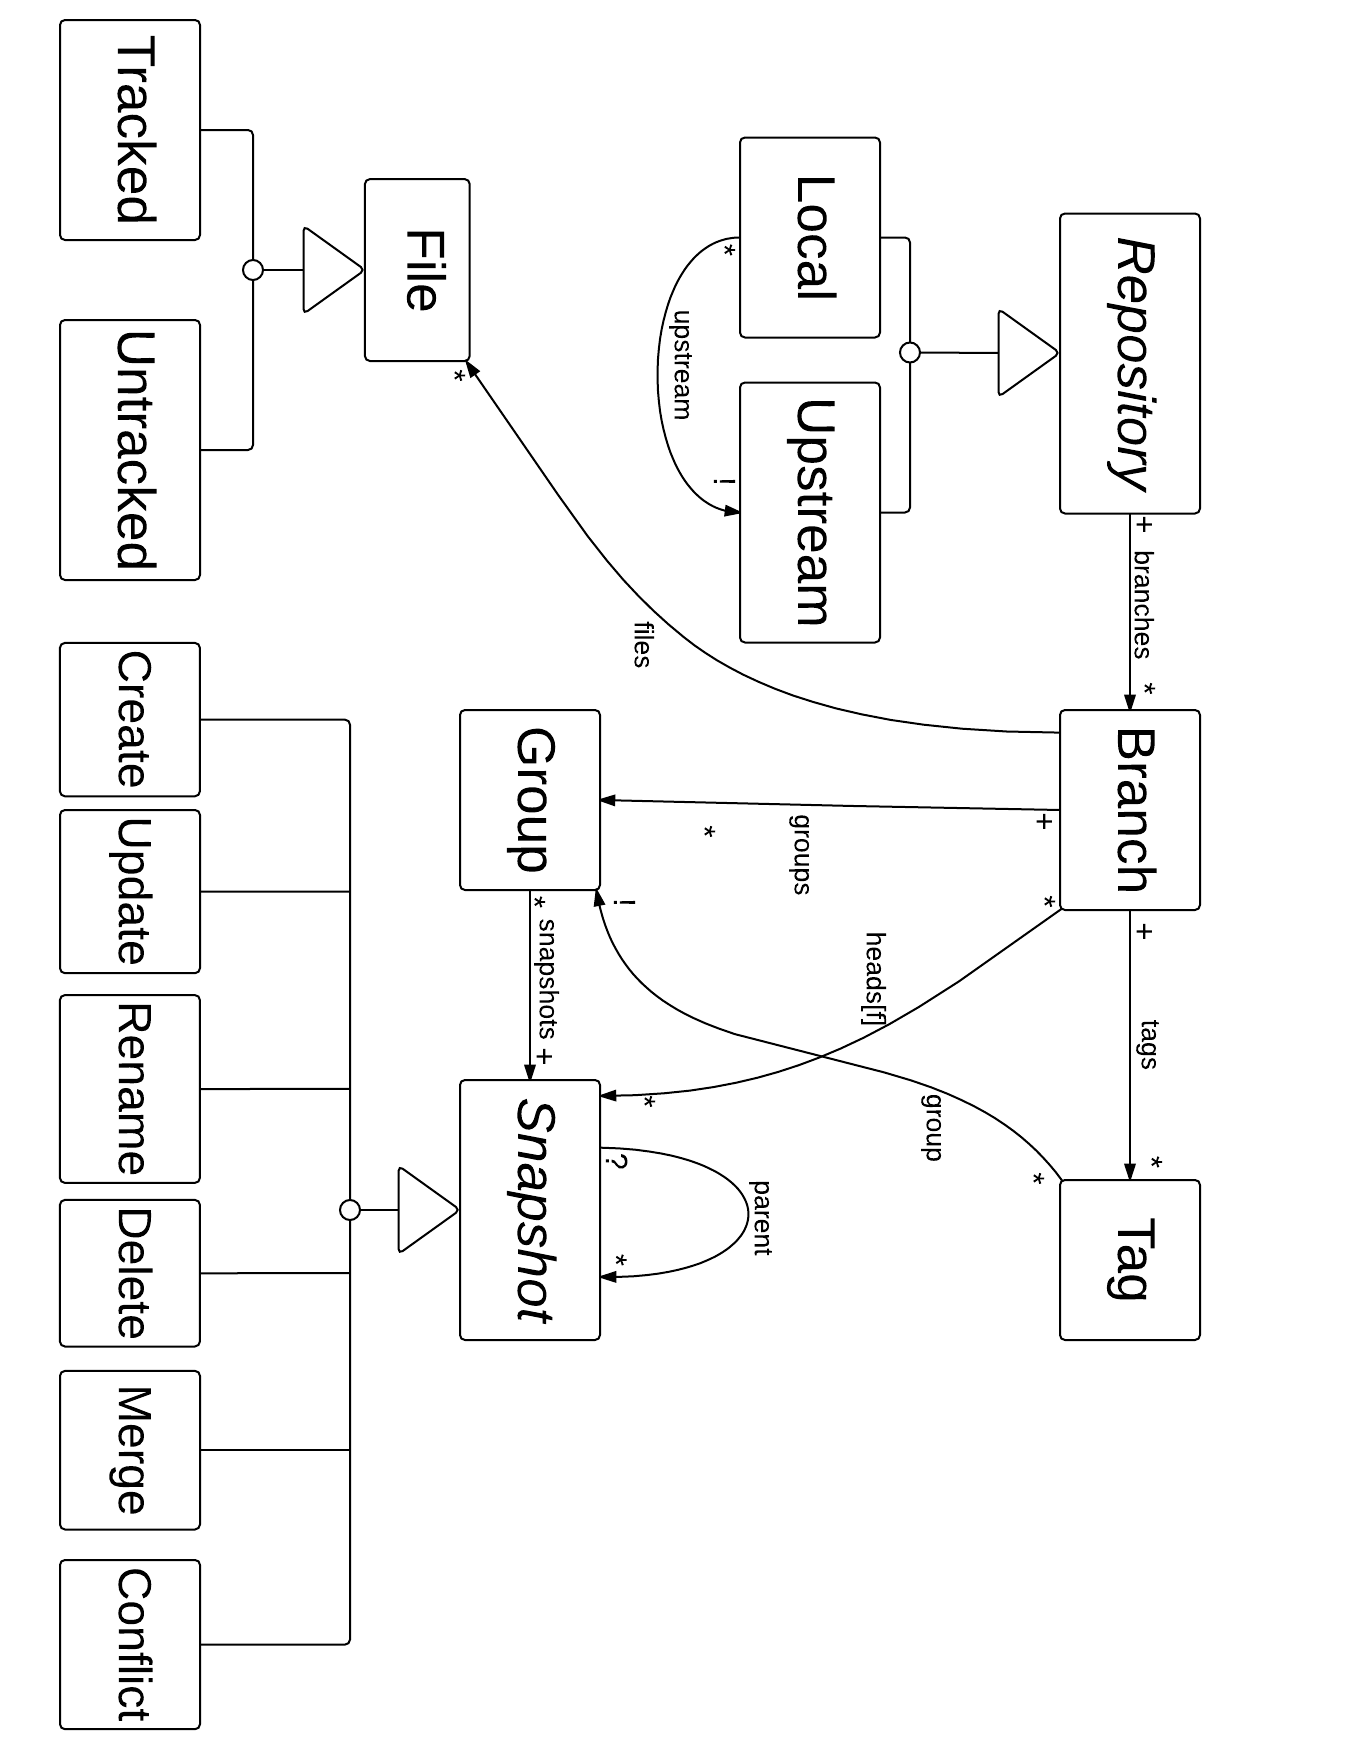
\includegraphics[max width= \linewidth]{ConceptModel}
\caption{Concept Model of Snapstore.}
\label{arm:fig1}
\end{figure}

\section{Data Storage - Snapshot}

Persistent data storage in Snapstore is achieved with the notion of a \textit{snapshot}. The snapshot is a saved state of a file. Snapshots record updates, renames, moves, deletes, along with merges and conflicts. Records of the many operations enable all VCS features of Snapstore. The \textit{head} snapshot for any given file is the most recent snapshot made for that file and the current content of that file. 

A snapshot is either a create, an update, a rename, a delete, a merge, or a conflict snapshot. This distinction dictates the values of the snapshot fields. Create snapshots have no parent. Update snapshots have a parent, a child, and content. Rename snapshots have a different filename than their parent. Delete snapshots have no content. Merge snapshots have more than one parent, and conflict snapshots are merge snapshots that have conflict markers in their data.

All snapshots have parent snapshots and child snapshots. The snapshots of a file are related by the graph they create with these parent/child relationships. This ordering forms the snapshot graph described in the tutorial section. The snapshot graph is guaranteed to be an in-order description of snapshots a specific client has made to a file in a branch. Each unique (branch, file) tuple is represented by its own snapshot graph. A snapshot can have multiple parents if it is the result of a merge operation.

Any file, identified by its snapshot graph, can either be tracked or untracked. Untracked files will not create snapshots and will not affect the local or upstream repositories.

\section{Grouping Changes - Group}

A \textit{group} is an assembly of related snapshots. A group must contain at least one snapshot, but there are no restrictions on what kinds of snapshots can be in the group or what their relationship must be. The same snapshot can exist in more than one group. It is up to the user to decide what makes a group of snapshots logically related. This allows flexibility in projects and development strategy.

Groups are an attribute of a specific branch. Even if a group contains the same snapshots across different branches, they are treated as different concepts because they exist on independent lines of development. They can be given names for identification for the user.

\section{Recording Coherent Points - Tag}

The notion of a \textit{tag} allows users to label logical milestones in their work. They describe groups but have an added function over a group's name: they describe the status of the group as representing a coherent point. Here, coherent means that the project is in a state that is ready for further development or work, though the definition will differ from team to team\cite{RossoJackson}. 

Tags will always describe groups that are perfectly vertical. That is, at most one snapshot from any file is in the group. An example of this is tagging every head snapshot in a branch at a given time with the tag ``Submitted to Scientific Journal'' or ``Version 1.0''.

Tags are also an attribute of the branch. This means that they must be created inside a of an independent line of development. They can be copied across branches when merging and cloning, but they stay a fundamental attribute of the branch concept.

\section{Support Parallel Lines - Branch}

In Snapstore, the concept of a \textit{branch} supports parallel and independent lines of development. These branches are completely separate from each other. They facilitate the appropriate partitioning of data.

The branch houses three of the other main concepts in Snapstore: snapshots, groups, and tags. All three of those concepts exist within the confines of a branch. All of these things together consitute a line of development, and so the branch is the conceptual representation of that line.

Branches make up a repository, whether that repository is local or upstream. Switching between them constitutes changing the line of development, project, folder, or anything that delineates the user's work. Switching between two branches on a single local repository that are stored on different upstreams has no averse effects due to their independence.

Branches can be merged together, synchronizing the parallel development. This simply involves combining each branch's individual snapshot, group, and tag data together as explained in chapter 2.2.3.

\section{Synchronize Changes of Collaborators - Upstream Repository}

Snapstore uses a centralized data storage system that holds all connected branch data, called an \textit{upstream repository}, or upstream for short. While users do not necessarily have to use an upstream for their local repository, it is the only way to collaborate with other users on any branch in that local repository.

Every local repository can have multiple upstreams. This allows the user to distribute where their snapshots, groups, and tags are saved and backed up. These upstreams can then be shared with other Snapstore users, provided that the upstream is connected to those users. 

All changes that occur at the branch level (branches, snapshots, groups, tags) are reflected in any connected upstream. There, the upstream can see if any other users have access to that branch and it can push the changes down to them.

\section{Disconnected Work - Local Repository}

The ability to leverage the benefits of a version control system without needing an internet or network connection is handled by the \textit{local repository}. The local repository affords all of the same relationships to other concepts as the upstream. That is, it is a collection of branches, which are in turn collections of snapshots, groups, and tags.

The local repository has one other important relationship, it can have zero or more upstreams attached to it. These upstreams are mirroring the data housed by the local repository.

\subsection{Discussion}

During the design process, there were many decisions made that had lasting tradeoffs for Snapstore. The main tradeoffs are explored below.

\subsubsection{Granularity of a Snapshot}

The decision of what a snapshot would represent was the first design decision we encountered. Either a snapshot could represent a file, or it could represent every file in a branch. In many VCSs such as Git and Mercurial, saving changes couples together the act of saving changes with the act of grouping changes, resulting in an overloaded concept \cite{Jackson}. We separated the saving of changes with grouping those changes, so the snapshot represents a single file.

Another reason the snapshot describes only a single file was that it was more intuitive to a typical user. If a user was to save a file and create a snapshot, they would expect that snapshot to relate to the object they just interacted with, that file. They would not expect it to relate to every file in the branch.

One downside of this approach is the additional computation needed to compute the current state of a branch. In Git, the current state is the head commit. In Snapstore, we need to calculate this by grabbing all of the head snapshots for a branch. This is typically trivial, so the tradeoff is beneficial.

\subsubsection{The Upstream}

Different version control systems and file sharing systems have their own ways of handling storage. Git, for example, use a decentralized storage system. Dropbox and SVN, on the other hand, use a centralized system. When deciding which model to use for our upstream, we looked at both models' pros and cons.

Snapstore uses a hybrid centralized/decentralized upstream model. On the surface, it is centralzied because all collaboration must take place via the upstream repository. That is, any data a user wants to collaborate on with another user must first go through a centralized repository.

But, Snapstore is also decentralized because users have a local repository, where actions can be made without requiring an active connection to the upstream. Snapstore users each have an entire history of their branch on their own system, just like in a decentralized version control system. Because of this, users can work offline, without checking out a central repository.

There are downsides to this hybrid model. Initially, there is only one upstream server, and so the location of the data is held by a single entity. If users want to set up their own server, they must use a machine to do so, and there is the overhead of setting up that server. Because there is no push/pull model in Snapstore, this machine must always be online in order to facilitate collaboration. Further, users cannot share directly with subsets of users on a given branch. They can, however, work around this limitation by creating new branches with new sets of users.

We used our goal of opt-in complexity to create a balance between the simplicity of a client/server, centralized model with some of the power of a decentralized system. The centralized model is easier for the majority of users to use, and it has a faster learning curve \cite{Brindescu}. In Snapstore, the data on the upstream is indeed ``blessed'', and so it is centralized. However, by offering a local repository alongisde and potentially independent from the upstream, Snapstore has some characteristics of a decentralized system.

\subsubsection{File Names}

Whether or not to make the file name a property of a file or the identifier for a file was an important decision for Snapstore. Systems like Git use the file name as an identifier for a file. Because of this decision, renames to a file are sometimes processed as deleting that file and creating a new file, causing much consernation among users (especially novices)\cite{RossoJackson}.

We wanted to be able to fully support renaming files in Snapstore, so file names in Snapstore are simply a property of the file. Each snapshot in a given snapshot graph will have the same file id. When branch merging occurs, only snapshot graphs with the same file id will be merged. The merge operation will look back over a file's two snapshot graphs for a common ancestor and perform a standard three-way merge. This allows Snapstore to accurately handle renames and merges.




\chapter{DESQ Algorithm}

\section{Shared Branches}

For Snapstore, we wanted users to be able to work on a shared branch. As described earlier, a shared branch is a line of development where a change from one user is propagated to all other users on that line as soon as a network connection is avilable. If there are multiple connected users on a shared branch, a change made by one of them should result in changes to the filesystems of all other users, so as to keep all local working directories consistent.

Furthermore, if there are multiple users on a shared branch, they should each be able to work independently, confident that any changes they make will not be lost. They should instead be intelligently inserted into the snapshot history of the branch. New changes can come in through the network while a user is working, but it should not affect their ability to send their own changes.

We have opted to use a last-write-wins methodology when saving changes between users because it would be an easier paradigm for non-technical users to understand. While this methodology might cause some offline edits to be very far removed from their original parent, we believe that it is appropriate for two reasons. First, in the current highly connected environment of today's computing, making that many offline edits is typically done by choice. Second, if offline edits are indeed an issue, Snapstore allows users to create a separate branch for highly disconnected development. 

\section{Network Issues}

The workflow described above can be difficult to maintain. Multiple users can be making multiple edits at the same time, increasing concerns of concurrency.  Furthermore, network concerns and partitions increase the difficulty and uncertainty of this problem. 

Imagine a user goes offline and makes multiple edits, all while their shared file is being written to by other, online users. Snapstore should be able to handle their reintroduction to the network without destroying the branch history. Simply trying to push these changes would be pushing an incorrect snapshot tree structure to the server. 

The most important invariant Snapstore must provide is a shared snapshot tree for its users. We take the approach that any data that reaches the upstream server and is accepted should be regarded as fact. That is, any snapshots that are confirmed by the server should not be undone. With this invariant, we can more adequately reason about how to propose a protocol algorithm for this process, an algorithm we call Distributed Event Sychronization Queue (DESQ).

\section{DESQ} 

We propose the DESQ algorithm. DESQ seeks to synchronize all queues - the server queue and all client queues - and to reach eventual consistency in the ordering of their events. For Snapstore, these events are snapshots and their queues are the snapshot trees for a particular file in a particular branch. 

These snapshots, at their core, describe a set of database actions and therefore describe an ordering that all parties can agree upon for system-wide accordance. When a new snapshot action in the database is triggered, that snapshot data is saved to the client queue. This queue, by itself, is a guaranteed in-order sequence of all snapshot database actions by the client. Each snapshot in the queue is related to its parent and its child by a pointer, and these pointers are used to detect inconsistencies. If the client is working by themselves, in their own branch, this queue will simply be mirrored by the server when the network in connected. If, however, the client is working with another client on the same snapshot tree, there may be concurrent events being sent to the server. This can result in issues of ordering across the system.

DESQ is an algorithm that begins when an inconsistency is detected in the system. This can happen in two ways. First, if a client creates an snapshot (that is unconfirmed by default), DESQ will begin to try to get the snapshot confirmed by the server and shared with all appropriate users. Second, if a client connects to the server and detects that changes have been made to the server's queue, it will pull in those changes to make the queues consistent. Once DESQ begins, it will not stop until the inconsistencies are resovled. 

Note that this protocol can proceed only when network connections between the server and client are open. If they are closed, the snapshots are queued in the client until the network is available. Then, they are processed in the same way. In the case of Snapstore, we use sockets for all network connections.

\subsection{Confirmed Snapshots}

In the most basic case, a single client is creating snapshots in their own queue, with no other users having access to that queue. The client will create a snapshot, the snapshot will be sent to the server, and the server will see that no additional snapshots have been added since the parent of this new snapshot. The server will add this snapshot to its version of the queue, set its confirmed flag to true, and send a response back to the client. On the client machine, the snapshot's confirmed flag will also be set to true, and the client can continue with full confidence that this event is consistent for all version of this particular snapshot queue.

\subsection{Receiving Snapshots From the Server}

When sharing a particular snapshot queue, more than one client will have read and write access to it. If a certain client sends a snapshot to the server and it is confirmed, then that snapshot must be propagated to all other involved clients. When a snapshot is confirmed, the server will find all clients that have access to that queue (all clients with access to the queue's branch). It will then push that snapshot, with the confirmed flag set to true, to those clients. Because this is a confirmed snapshot coming from the server, the other clients can append this snapshot to their own queue, knowing that all queues are still consistent in the system.

When a snapshot comes in from the server to the client, to be inserted into the queue, its parent snapshot should be the end of the client's queue. This is because the rejected snapshot protocol (which can be happening simultaneously) will already be including the snapshot with its response, so there's no need to apply it in this case. 

\subsection{Rejected Snapshots}

To combat the concurrency issues, DESQ takes an approach that results in a last-write-wins methodology. When a snapshot is logged to the client’s queue, it is sent to the server to be verified. The server then verifies whether or not it has seen a different snapshot from another client. This is done by checking the parent of the incoming snapshot. If the parent of the incoming snapshot matches the last known confirmed snapshot on the server, it is allowed in. If another client has already sent a snapshot that has been confirmed, then that snapshot will not match the incoming snapshot's parent.

If the server has seen other snapshots, making the server queue inconsistent with the client queue, it rejects the client's snapshot. The rejected snapshot then goes back to the client, along with the snapshot(s) that caused the rejection. These additional snapshots are inserted before the rejected snapshot in the client's event queue, and the rejected snapshot is queued again for confirmation at the front of the queue and sent to the server, starting DESQ all over again. 

Because the rejected snapshot is sent to the front of the queue of snapshots to be sent to the server, this process can continue without disrupting the inherent correct ordering of snapshots for a single client. So, if a client has made multiple offline edits, only the first of those will trigger the rejection. The snapshots causing the rejection will be inserted, and the process will start over with that first snapshot.

Furthermore, this robust way of handling rejections allows for the system to handle consecutive rejections. This can occur in the case where other clients are sending snapshots to the server while another clients' snapshots are beign rejected.

\subsection{Duplicate Events}

In the case of network outages, it could be the case the client goes down before the server can respond that it has received a valid snapshot. In this case, when the client comes back online, it will simply retry to send that snapshot. Since that snapshot already exists in the server’s queue of snapshots, it will simply respond that it has already received the snapshot. This will allow the client to confirm the snapshot as valid while not having to re-push the snapshot to the server.



\chapter{Implementation}

This chapter details the implementation of Snapstore. This includes data structures, interface images, and the synchronization algorithm. 

Snapstore was built to be cross-platform using Electron\footnote{http://electron.atom.io/}. We used web sockets\footnote{www.socket.io} for networking. Once a client is connected over a socket, Snapstore can constantly pull in and push out new snapshots that come in from that user and from other users. Sockets provide the additional benefit of allowing us to group users. We used this functionality to make ``rooms'' of users that have read and write access to a specific branch. Pushing changes on that branch out to those users is simple with sockets.

\section{Data Structures}

\subsection{Client}

Each local repository on the client has its own Mongo\footnote{https://www.mongodb.com/} database. Each database has a collection of snapshots, branches, groups, tags, and events. It also has one snapstore document and a binary large object (blob) collection. A data model representing each data structure and its attributes is shown in figure 4-1.

\begin{figure}
\includegraphics[max width= \linewidth]{DataModel}
\caption{Snapstore client data model.}
\label{arm:fig1}
\end{figure}

When a file is saved, the resulting snapshot must first decide what kind of snapshot it is. Whether it is a create, update, rename, delete, merge, or conflict snapshot dictates how it will populate its data fields. A create snapshot, for example, has no parent snapshot. When a snapshot is created, it is added to the snapshot collection, and its branch updates its head snapshots to include the new snapshot, while removing its parent. To read the history of a file, the head snapshot of the file is located, and the rest is found by searching backwards through the snapshot graph.

If two snapshots have the same content, they point to the same blob data in the blob collection to save space. This blob collection holds hashes of the content along with the binary content.

When a new branch is created, it is added to the database with only a name. If, however, it was cloned from another branch, the cloned branch will point to all head snapshots, groups, and tags from the original branch. When switching to a branch, the heads snapshots for the target branch are read and applied to the Snapstore folder.

The event collection stores all of the snapshots, groups, and tag events on the client that have not been confirmed by the server. As these events are confirmed, they are erased from the collection.

\subsection{Upstream}

On the upstream server, the snapshot, branch, group, tag, and content data structures are the exact same as those on the client. They are kept consistent with each local repository when a socket connection is open. A model of the data structures on the upstream is shown in figure 4-2.

\begin{figure}
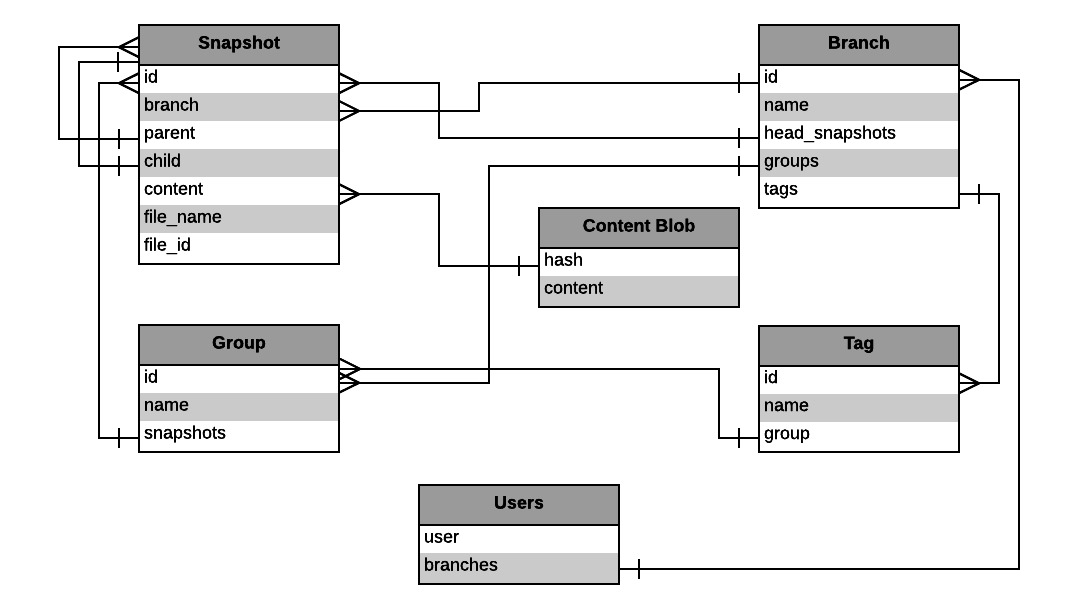
\includegraphics[max width= \linewidth]{DataModelServer}
\caption{Snapstore server data model.}
\label{arm:fig1}
\end{figure}

The user model on the server is a mapping of users to branches to which they have access. When a user shared a branch with another user, that branch is added to this mapping for that user. The server uses this mapping to share data with the appropriate users.

\section{User Interface}

**Pictures will go in here when the UI is done.**

\section{Keeping Data in Sync}

In Snapstore, users can work on a shared branch. As described in section 2.2.3, a shared branch is a line of development where a change from one user is propagated to all other users who are collaborators on that branch, keeping all of their Snapstore folders consistent.

However, this workflow can be difficult to maintain. Multiple users can be making edits at the same time, increasing concurrency issues. If two snapshots are made at the same time, there needs to be a way to resolve the snapshot graph. Also, a user can go offline and create snapshots, while their shared snapshot graphs are being written to by other, online users. Snapstore should be able to handle their reintroduction to the network without destroying the snapshot graph.

It is also important to maintain the ordering of events created by a single user. If a user creates a snapshot and then creates a group with that snapshot it in, it is necessary to send those two events in order to the server. Otherwise, the server might, for example, try to create a group containing a snapshot that doesn't exist.

We take the approach that any data that reaches the upstream server and is confirmed should be regarded as fact; it should never be undone. With this invariant, we designed a protocol algorithm for this process, called Distributed Event Synchronization Queue (DESQ).

\begin{center}
\begin{algorithm}[h]
\caption{DESQ}\label{euclid}
\begin{algorithmic}[1]
\Procedure{Client-DESQ}{}
\State $\textit{events} \gets \text{collection of }\textit{Events}$
\State $\textit{socket} \gets \text{server socket connection}$
\While {\emph{events} not empty}
\State $socket\text{.send(}events(0)\text{)}$
\EndWhile
\Loop{ on \emph{socket}.response(\emph{response, message})}:
\State Save \emph{response}
\If {$message == \text{"Confirm" or "Duplicate"}$}
\State \emph{events}.remove(\emph{events}(0))
\EndIf
\If {$message == \text{"Reject"}$}
\State $events\text{(0).data.parent} = response\text{(-1)}$
\EndIf
\EndLoop
\EndProcedure
\end{algorithmic}
%%%%%%%%%%%%%%%%%%%
\begin{algorithmic}[1]
\Procedure{Server-DESQ}{}
\State $\textit{db} \gets \text{MongoDB}$
\State $\textit{socket} \gets \text{client socket connection}$
\Loop{ on \emph{socket}.receive(\emph{event})}:
\If {$\textit{event} \text{.data.id in } \textit{db}$}
\State return $socket\text{.send(}event, \text{"Duplicate")}$
\EndIf
\If {$\textit{event}\text{.type } != \text{snapshot}$}
\State $event\text{.confirmed} \gets \text{True}$
\State $socket\text{.send(}event, \text{"Confirm")}$
\State return $socket\text{.room.send(}event, \text{"New Event")}$
\Else
\If {$event\text{.data.parent is head snapshot}$}
\State $event\text{.confirmed} \gets \text{True}$
\State $socket\text{.send(}event, \text{"Confirm")}$
\State return $socket\text{.room.send(}event, \text{"New Event")}$
\Else
\State $conflictSnapshots \gets \text{All snapshots between }event\text{.parent and }head$
\State return $socket\text{.send(}conflictSnapshots\text{,"Reject")}$
\EndIf
\EndIf
\EndLoop
\EndProcedure
\end{algorithmic}
\end{algorithm}
\end{center}

Each client has their own ordering of events, or database operations, that are stored in a client queue until they are confirmed by the server. The DESQ algorithm seeks to reach eventual consistency between these queues so that every client on a shared branch has the same data.

DESQ begins when an inconsistency is detected in the system. This can happen in two ways. First, if there is an event in the client's event queue, the algorithm will try to get that event confirmed by the server and shared with all appropriate users. Second, if a client connects to the server and detects that changes have been made, it will pull in those changes. Note that this protocol can proceed only when a network connection between the server and client is open. If they are closed, the events are queued until the network is available.

%Confirm + Duplicate
This algorithm pushes these events one at a time to the server repository. Events are confirmed if they can be applied to the server without causing any conflicts in the data. On the client, when an event is confirmed, it is removed from the event queue. Events also have a unique ID, so duplicate events can be caught and handled the same way.

%Push
When a client sends an event to the server and it is confirmed, the event must be propagated to all other collaborators. The server will find all clients that have access to that event's branch and send it to them. Because this is a confirmed event coming from the server, the other clients can apply this event to their local repository without adding it to their event queue.

%Reject
Snapshots are the only type of event that can cause a conflict, due to their inclusion in an ordered snapshot graph. All clients with access to this snapshot graph must agree on its order. The server will reject a client's snapshot event if the snapshot's snapshot graphs on the server and client are inconsistent. The rejected snapshot returns to the client with snapshots that will fix the inconsistencies.

In Git terms, if there is a conflict, the snapshot graph rebases and Snapstore tries to push that snapshot again. The rebasing keeps the snapshot graph and the workflow for the branch linear. However, while Git creates new commits during a rebase, Snapstore uses existing snapshots.

This protocol allows the system to handle consecutive rejections. This can occur when other clients are sending snapshot events to the server while another client's event is being rejected.



\chapter{Conclusion}

Snapstore is a version control system that tries to bridge the gap between version control systems and file syncing systems to being the best of both worlds to users. Its motivating purpose is to be simple enough for every user and powerful enough for every user. By following the theory of conceptual design, we believe Snapstore's design has acheived that.

Snapstore still has implementation-specific needs and flaws which will need to be addressed before it is widely used. By open-sourcing this project, we hope it development will continue and its full design is realized. 
\appendix
\chapter{Tables}

\begin{table}
\caption{Armadillos}
\label{arm:table}
\begin{center}
\begin{tabular}{||l|l||}\hline
Armadillos & are \\\hline
our	   & friends \\\hline
\end{tabular}
\end{center}
\end{table}

\clearpage
\newpage

\chapter{Figures}

\vspace*{-3in}

\begin{figure}
\vspace{2.4in}
\caption{Armadillo slaying lawyer.}
\label{arm:fig1}
\end{figure}
\clearpage
\newpage

\begin{figure}
\vspace{2.4in}
\caption{Armadillo eradicating national debt.}
\label{arm:fig2}
\end{figure}
\clearpage
\newpage

%% This defines the bibliography file (main.bib) and the bibliography style.
%% If you want to create a bibliography file by hand, change the contents of
%% this file to a `thebibliography' environment.  For more information 
%% see section 4.3 of the LaTeX manual.
\begin{singlespace}
\bibliography{main}
\bibliographystyle{plain}
\end{singlespace}

\end{document}

